\documentclass[12pt, twoside]{article}
\input{../preamble}

\title{PreCalculus}
\author{Chris Huson}
\date{March 2023}

\fancyhead[LE]{\thepage}
\fancyhead[RO]{\thepage \\ Name: \hspace{3cm} \,\\}
\fancyhead[LO]{BECA / Huson / Unit 11: Calculus \\* 4 April 2023}

\begin{document}

\subsubsection*{11.4 Quiz: Derivatives}
Use your own notebook, but no calculators or computers

\begin{enumerate}[itemsep=2cm]

\subsubsection*{State the derivative of a polynomial function}
\item $f(x)=x^3+4x^2$
\item $f(x)=x^5-3x^4+2x^2$ \par \vspace{2cm}

\subsubsection*{Evaluate a function and its derivative at a given point}

\item Given $f(x)=2x^3-5x^2$
\begin{enumerate}[itemsep=2cm]
    \item Find $f(1)$
    \item Find $f'(1)$
\end{enumerate} \vspace{2cm}

\item The graph shows the exponential function $\displaystyle f(t)=1200 \times \left( 1+0.18 \right)^t$ representing 18\% annual growth rate over $t$ years.
\begin{multicols}{2}
    \begin{enumerate}[itemsep=1cm]
        \item Write down the initial deposit in the account.
        \item What is the annual interest rate?
        \item Approximately how much will the account hold at the end of ten years?
        \item When will the balance be \$1,400?
    \end{enumerate}
    \begin{center}
    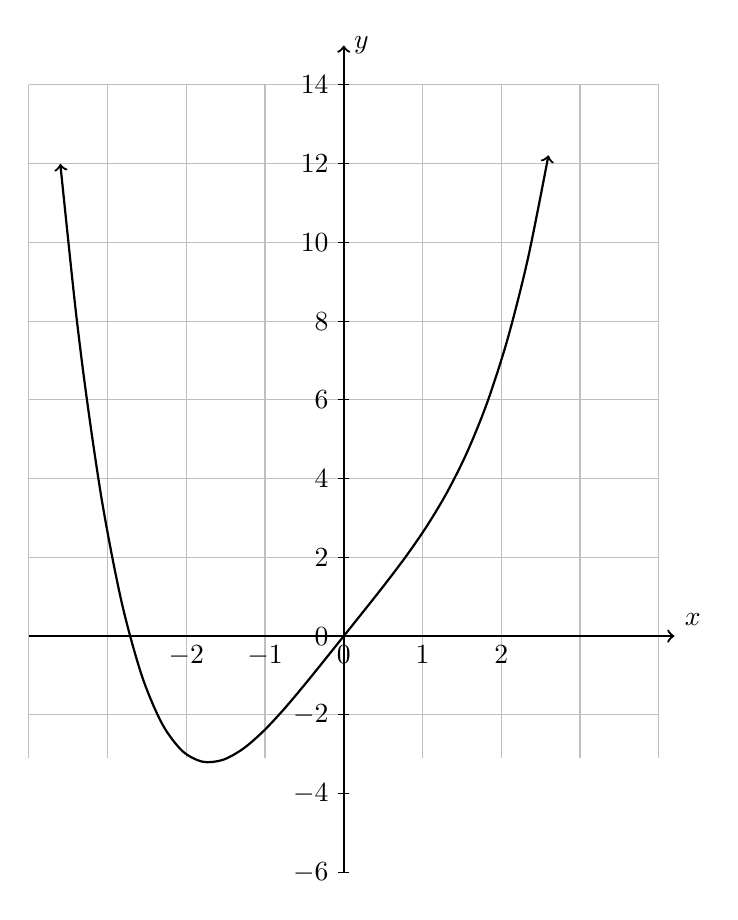
\begin{tikzpicture}[x=2cm, y=0.5cm, scale=1]
        \draw [thin, color=lightgray, xstep=1.0cm,ystep=1.0cm] (-2,-3.1) grid (2,14);
        \draw [thick, ->] (-2,0) -- (+2.1,0) node [above right]{$x$};
        \draw [thick, ->] (0,-6) -- (0,15) node [right]{$y$};
        \foreach \x in {-2,...,2}
            \draw (\x cm,0) -- (\x cm,0) node[below] {$\x$};
        \foreach \y in {-6,-4,...,14}
            \draw[shift={(0,\y)}] (2pt,0pt)--(-2pt,0pt) node[left]{$\y$};

        \draw [thick,<->,smooth,domain=-1.8:1.3] plot(\x,{(2*\x*\x*\x*\x+5*\x)});
    \end{tikzpicture}
    \end{center}
    \end{multicols}

\newpage
\item The graph shows the exponential function $\displaystyle FV=1,100 \times \left( 1+\frac{6.125}{100} \right)^t$ representing the balance of an investment account earning a fixed rate of interest over $t$ in years.
\begin{multicols}{2}
    \begin{enumerate}[itemsep=1cm]
        \item Write down the initial deposit in the account.
        \item What is the annual interest rate?
        \item Approximately how much will the account hold at the end of ten years?
        \item When will the balance be \$1,400?
    \end{enumerate}
    \begin{center}
    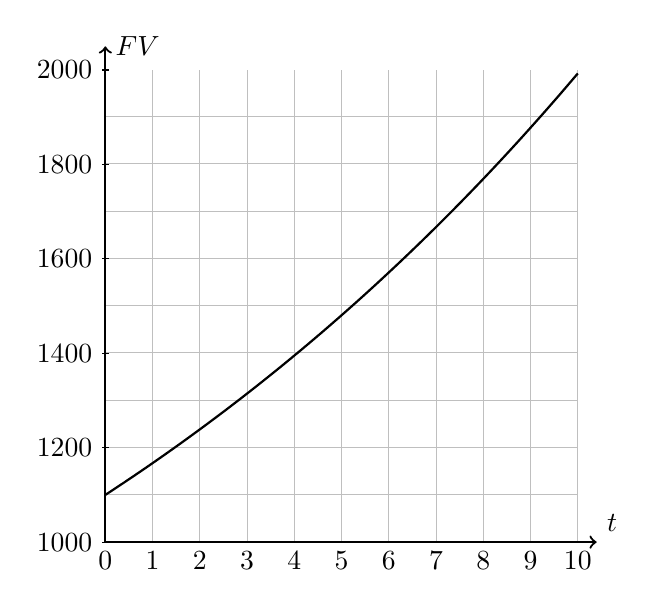
\begin{tikzpicture}[x=1cm, y=0.01cm, scale=0.6]
        \draw [thin, color=lightgray, xstep=1.0cm,ystep=1.0cm] (0,1000) grid (10,2000);
        \draw [thick, ->] (0,1000) -- (+10.4,1000) node [above right]{$t$};
        \draw [thick, ->] (0,1000) -- (0,2050) node [right]{$FV$};        \foreach \x in {0,1,...,10}
            \draw (\x cm,1000) -- (\x cm,1000) node[below] {$\x$};
        \foreach \y in {1000,1200,...,2000}
            \draw[shift={(0,\y)}] (2pt,0pt)--(-2pt,0pt) node[left]{$\y$};

        \draw [thick, smooth,domain=0.:10] plot(\x,{1100*(1.06125^\x)});
    \end{tikzpicture}
    \end{center}
    \end{multicols}

\end{enumerate}
\end{document}



